%! TeX program = lualatex
\documentclass[../main.tex]{subfiles}
\begin{document}
\begin{lesson}{Limits at Infinity}
  Let's begin by making sense of the \emph{idea} behind the \hlmain{limit at infinity}. There is an apple a metre away from us. We start by taking a step \(1/2\) metre away towards the apple. Each subsequent step is half the length of the previous one. 

  \begin{center}
    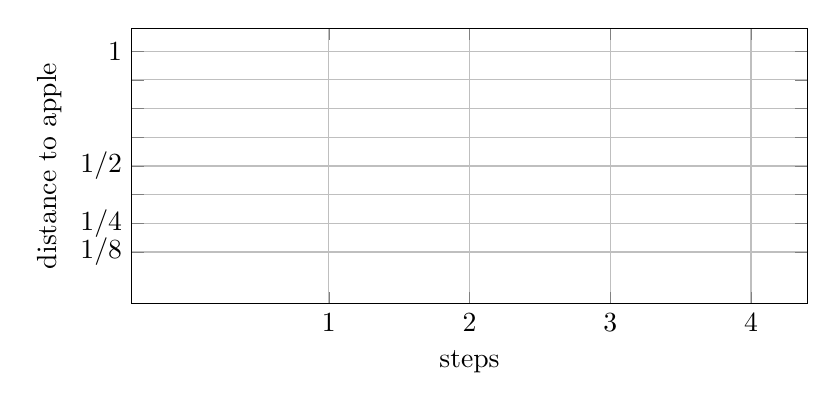
\begin{tikzpicture}[scale=1]
      \begin{axis}[xmin=0, xmax=4, ymin=0, ymax=1, xlabel={steps}, ylabel={distance to apple}, xtick={1,2,3,4}, ytick={1/8, 2/8,..., 1}, yticklabels={\(1/8\),\(1/4\),,\(1/2\),,,,\(1\)}, axis equal image=false, width=4in, height=2in, grid=major, enlargelimits]
    \end{axis}
    \end{tikzpicture}
  \end{center}

  \faComment{} Can we get as close to the apple as we want?

  \faComment{} If we can take infinitely many steps, can we reach the apple?
  \blanklines{5}


  \begin{mdframed}[style=withref-compact]
    If the values of \(f(x)\) become arbitrarily close to \(L\) as \(x\) becomes sufficiently large, we say \(f\) has \hlmain{a limit at (positive) infinity} and write 
    \[
      \lim_{x \to \infty} f(x) = L.
    \]

    If the values of \(f(x)\) become arbitrarily close to \(L\) as \(x\) becomes sufficiently small, we say \(f\) has \hlmain{a limit at negative infinity} and write
    \[
      \lim_{x \to -\infty} f(x) = L.
    \]

    If \(\lim_{x \to \infty} f(x) = L\) or \(\lim_{x \to -\infty} f(x) = L\), and \(L\) is a real number, then we say the line \(y = L\) is a \hlmain{horizontal asymptote} of \(f\).

    \textbook{Page 408}
  \end{mdframed}
  \clearpage

  \begin{example}
    Use the above definitions to help you sketch example functions with prescribed limits and horizontal asymptotes. Label your graphs with the name of the function. 

    Each part has (a lot) more than one right answer. 

    \begin{enumerate}[label=\(f_{\arabic*}\)]
      \item satisfies \(\lim_{x \to \infty} f_{1}(x) = -2\) and \(\lim_{x \to -\infty} f_{1}(x) = 3\).
      \item satisfies \(\lim_{x \to \infty} f_{2}(x) = \infty\) and \(\lim_{x \to -\infty} f_{2}(x) = 5/3\).
        \begin{center}
          \includegraphics{../standalones/build/plot_limit_at_infinity_exercise}
          \qquad
          \includegraphics{../standalones/build/plot_limit_at_infinity_exercise}
        \end{center}

      \item has no limits at both infinities, and \(\lim_{x \to -\infty} f_{3}(x)\) is not an infinity. 
      \item has exactly one horizontal asymptote.

        \begin{center}
          \includegraphics{../standalones/build/plot_limit_at_infinity_exercise}
          \qquad
          \includegraphics{../standalones/build/plot_limit_at_infinity_exercise}
        \end{center}

      \item has two different horizontal asymptotes.
      \item is bounded between \(y = -2\) and \(y = 2\) but has NO horizontal asymptote.

        \begin{center}
          \includegraphics{../standalones/build/plot_limit_at_infinity_exercise}
          \qquad
          \includegraphics{../standalones/build/plot_limit_at_infinity_exercise}
        \end{center}
    \end{enumerate}

  \end{example}
  \clearpage

  \begin{example}[Make your own exam!]
    Challenge yourself and other to sketch a function \(f(x)\) satisfying a random subset of properties from below, \emph{or} \hlsupp{explain} why such function does not exist!

    Rinse and repeat. For more practice, sketch a random function and fill in the blanks! 

    \begin{enumerate}
      \item Its \(y\)-intercept is \underline{\hspace{1in}} (pick a constant)
      \item Its \(x\)-intercepts are \underline{\hspace{1in}} (\emph{non-existent} or pick one or more constants)
      \item Its graph passes through \underline{\hspace{2in}} (pick one or more points on the plane)
      \item It has \underline{\hspace{1in}} horizontal asymptote (pick from \emph{no}, \emph{one}, \emph{exactly one}, \emph{two}, \emph{exactly two})
      \item Its horizontal asymptotes are \underline{\hspace{1in}} (\emph{non-existent} or pick one or more constants)
      \item Its vertical asymptotes are \underline{\hspace{1in}} (\emph{non-existent} or pick one or more constants)
      \item \(\lim_{x \to \infty} f(x) = \underline{\hspace{1in}}\) (pick a constant or from \emph{does not exists}, \(\infty\), \(-\infty\).)
      \item \(\lim_{x \to -\infty} f(x) = \underline{\hspace{1in}}\) (pick a constant or from \emph{does not exists}, \(\infty\), \(-\infty\).)
      \item Its range is \underline{\hspace{1in}} (pick a finite or an infinite interval)
    \end{enumerate}
  \end{example}

  \begin{center}
    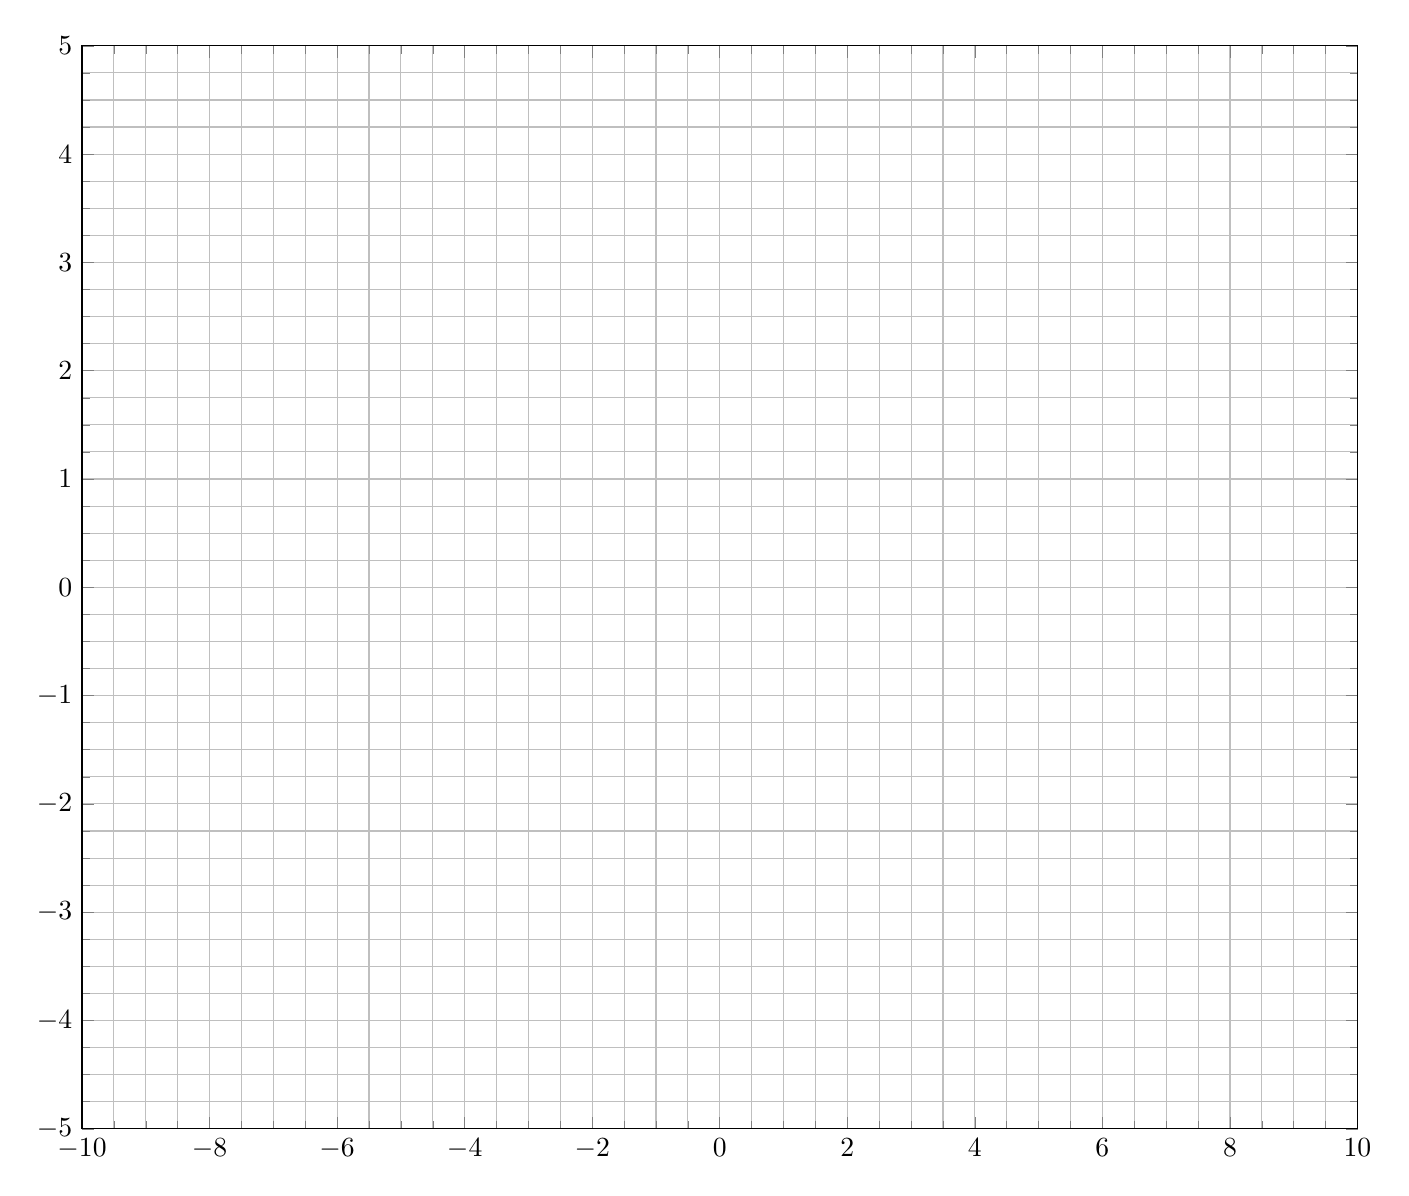
\begin{tikzpicture}[scale=1]
      \begin{axis}[ymin=-5, ymax=5, xmin=-10, xmax=10, grid=both, minor tick num=3, width=7in]

      \end{axis}
    \end{tikzpicture}
  \end{center}
  
  \bigskip

  \begin{example}
    What can we deduce from knowing \(\lim_{x \to -\infty} f(x)\) exists? 

    \begin{itemize}
      \item[(a)] \(f\) is not increasing on some interval \((-\infty, a)\)
      \item[(b)] \(f\) is not decreasing on some interval \((-\infty, b)\)
      \item[(c)] \(f\) is not oscillating on some interval \((-\infty, c)\)
      \item[(d)] \(f\) is increasing on some interval \((-\infty, \alpha)\)
      \item[(e)] \(f\) is decreasing on some interval \((-\infty, \beta)\)
    \end{itemize} 
  \end{example}
  \clearpage

  We turn to finding horizontal asymptotic from algebraic expressions of functions. Equation~\eqref{eq:horizontal-asymptote-flip} ``flips'' a negative infinity to a positive infinity and is quite useful.
  \begin{equation} \label{eq:horizontal-asymptote-flip}
    \lim_{x \to -\infty} f(x) = \lim_{x \to \infty} f(-x)
  \end{equation}
  \begin{center}
    \begin{tikzpicture}[scale=1]
      \begin{axis}[ymin=-pi/2, ymax=pi/2, xmin=-3, xmax=3, enlargelimits]
        \addplot[thick, domain=0:4] {atan(x)};
        \addplot[thick, domain=-4:0] {atan(x)};
        \addplot[dashed] coordinates {(-4,  pi/2) (4, pi/2)};
        \addplot[dashed] coordinates {(-4, -pi/2) (4,-pi/2)};
        \node[below right] at (axis cs:0,pi/2) {\scriptsize \(y = \pi/2\)};
        \node[above right] at (axis cs:0,-pi/2) {\scriptsize \(y = -\pi/2\)};
        \node at (axis cs:3,1) {\scriptsize \(\arctan(x)\)};
      \end{axis}
    \end{tikzpicture}
    \hspace{1cm}
    \begin{tikzpicture}[scale=1]
      \begin{axis}[ymin=-pi/2, ymax=pi/2, xmin=-3, xmax=3, enlargelimits]
        \addplot[thick, domain=0:4] {atan(-x)};
        \addplot[thick, domain=-4:0,] {atan(-x)};
        \addplot[dashed] coordinates {(-4,  pi/2) (4, pi/2)};
        \addplot[dashed] coordinates {(-4, -pi/2) (4,-pi/2)};
        \node[below right] at (axis cs:0,pi/2) {\scriptsize \(y = \pi/2\)};
        \node[above right] at (axis cs:0,-pi/2) {\scriptsize \(y = -\pi/2\)};
        \node[left] at (axis cs:3.5,1) {\scriptsize \(\arctan(-x)\)};
      \end{axis}
    \end{tikzpicture}
  \end{center}

  \begin{example}
    Find horizontal asymptotes of \(e^{x}\).

    \blanklines{15}
  \end{example}

  All limit laws applies to limits at infinity, but we often need to reorganize functions by \hlmain{factoring out its dominant (fastest growing) term}. We demonstrate the idea in Example~\ref{ex:dom-term-intro} before introducing the general problem-solving principle.

  \begin{example}\label{ex:dom-term-intro}
    Evaluate \(\lim_{x \to \infty} \frac{(2x-1)^{2} + 1}{x^{2}}\) or explain why it does not exist.

    \blanklines{15}
  \end{example}
  \clearpage

  Because of Equation~\eqref{eq:horizontal-asymptote-flip} on page~\pageref{eq:horizontal-asymptote-flip}, a limit at the negative infinity can be ``flipped'' to a limit at the positive infinity limit. 

  Therefore, we only need to discuss \hlmain{the problem-solving principle} for evaluating \(\lim_{x \to \infty} f(x)\). In general, \(e^{x}\) dominates (grows faster) than any power function as \(x \to \infty\). Among power functions with positive exponents, the one with the largest the exponent dominates as \(x \to \infty\).

  After factoring out the dominant terms and cancellations, we use the limit laws and one of these.
  \begin{align*}
    \lim_{x \to \infty} e^{x} &= \infty, & \lim_{x \to \infty} x^{(\text{positive constant})} &= \infty, & \quad \lim_{x \to \infty} \frac{1}{x^{(\text{negative constant})}} &= \infty \\
    \lim_{x \to \infty} \frac{1}{e^{x}} &= 0, & \lim_{x \to \infty} \frac{1}{x^{(\text{positive constant})}} &= 0, & \quad \lim_{x \to \infty} x^{(\text{negative constant})} &= 0
  \end{align*}

  \begin{example}
    Let \(f(x) = \frac{\sqrt[3]{-5x^{5} + 3x} - 2}{x^{2} + 1}\). 
    Evaluate \(\lim_{x \to \infty} f(x)\) and \(\lim_{x \to -\infty} f(x)\). 

    \blanklines{25}
  \end{example}

  \begin{example}
    Evaluate \(\lim_{x \to \infty} \frac{2x^{3} + 2}{\sqrt{x + 1}}\).
    \blanklines{10}
  \end{example}
  \clearpage

  \begin{example}
    Evaluate \(\lim_{x \to \infty} \frac{1}{x} \sin(x)\).

    {\scriptsize Hint: Use the squeeze theorem. Notice we only need to consider the case when \(x\) is positive because \(x \to \infty\). The solution is relatively straightforward and not very long.}

    \blanklines{25}
  \end{example}

  If we want to be a bit tricky, then we could put negative exponents in functions.  In such case, turn all negative exponents into fractions and reorganize the expression before factoring.
  \begin{example}[Algebra skill practice]
    Evaluate \(\lim_{x \to \infty} \frac{x^{-5/2} + 3x^{2}}{x^{2} - 1/2}\). 
  \end{example}
\end{lesson}
\end{document}

